  \chapter{Introduction}
\label{chapter_introduction}
%% Start the actual chapter on a new page.
\newpage

\noindent

Once upon a time, there was the evolution of all life on
Earth. Let me tell the simplified version of this story and how
to put this into figures called phylogenies, before moving to the
more complex details. 
The formation of the Earth began approximately 4.5 billion years 
ago (\cite{dalrymple2001age}).
From an evolutionary biologists' point of view, 
this was a dull time,
until the first living organism appeared.

This First Universal Common Ancestor (FUCA) came into existence at least 
3.48 billion years ago (\cite{noffke2013microbially}). 
FUCA may not have been alone, but these other early life forms went extinct 
\footnote{by definition!} and are ignored in this story .
We can depict the evolutionary history of FUCA at that point in time
with figure \ref{fig:t_0}.

\begin{figure}[H]
  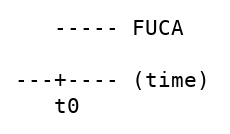
\includegraphics[width=0.3\textwidth]{t_0.png}
  % 
  %    ----- FUCA
  %
  % ---+---- (time)
  %    t0
  %
  \caption{
    Evolutionary history of the First Universal Common Ancestor (FUCA).
    Time goes from past (left) towards the present (right).
  }
  \label{fig:t_0}
\end{figure}

One unknown day, the descendants of FUCA became
dissimilar enough to say that the one species called FUCA 
gave rise to two species (note the difficulty in determining what 
a species is at that time!).
This event doubled the biodiversity on Earth.
The two species that FUCA evolved into will be called species A and B. Species A and B are sister species. 
We can depict the evolutionary
history of these two species in figure \ref{fig:t_1}.

\begin{figure}[H]
  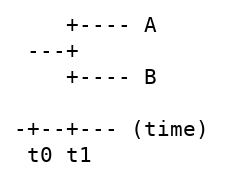
\includegraphics[width=0.3\textwidth]{t_1.png}
  %
  %     +---- A
  %  ---+
  %     +---- B
  %
  % -+--+--- (time)
  %  t0 t1
  %
  \caption{
    Evolutionary history of the two descendants of FUCA.
    Time goes from past (left) towards the present (right).
  }
  \label{fig:t_1}
\end{figure}

Both species A and B have their unknown histories.
One of them may have gone extinct, as extinction 
is a common event: it is estimated that more than 99\% 
of all species that has ever lived on Earth has gone 
extinct (\cite{newman1997model}).
Alternatively, they may have given rise to new species, but these
are just as likely to go extinct.
For this story, we will assume A and/or the clade of its descendant species went
extinct and that species B created a sister species C. 
Species B and C gave rise to all contemporary biodiversity. 
This ancestor of species B and C 
is called the Last Universal Common Ancestor, or LUCA.
LUCA is estimated to have lived between 3.48 (\cite{noffke2013microbially}) 
and 4.5 (\cite{betts2018integrated}) billions of years ago.
We can depict the evolutionary
history of LUCA in figure \ref{fig:t_3}.
Here, billions of years ago, is where the story ends 
and we will move on to the present.

\begin{figure}[H]
  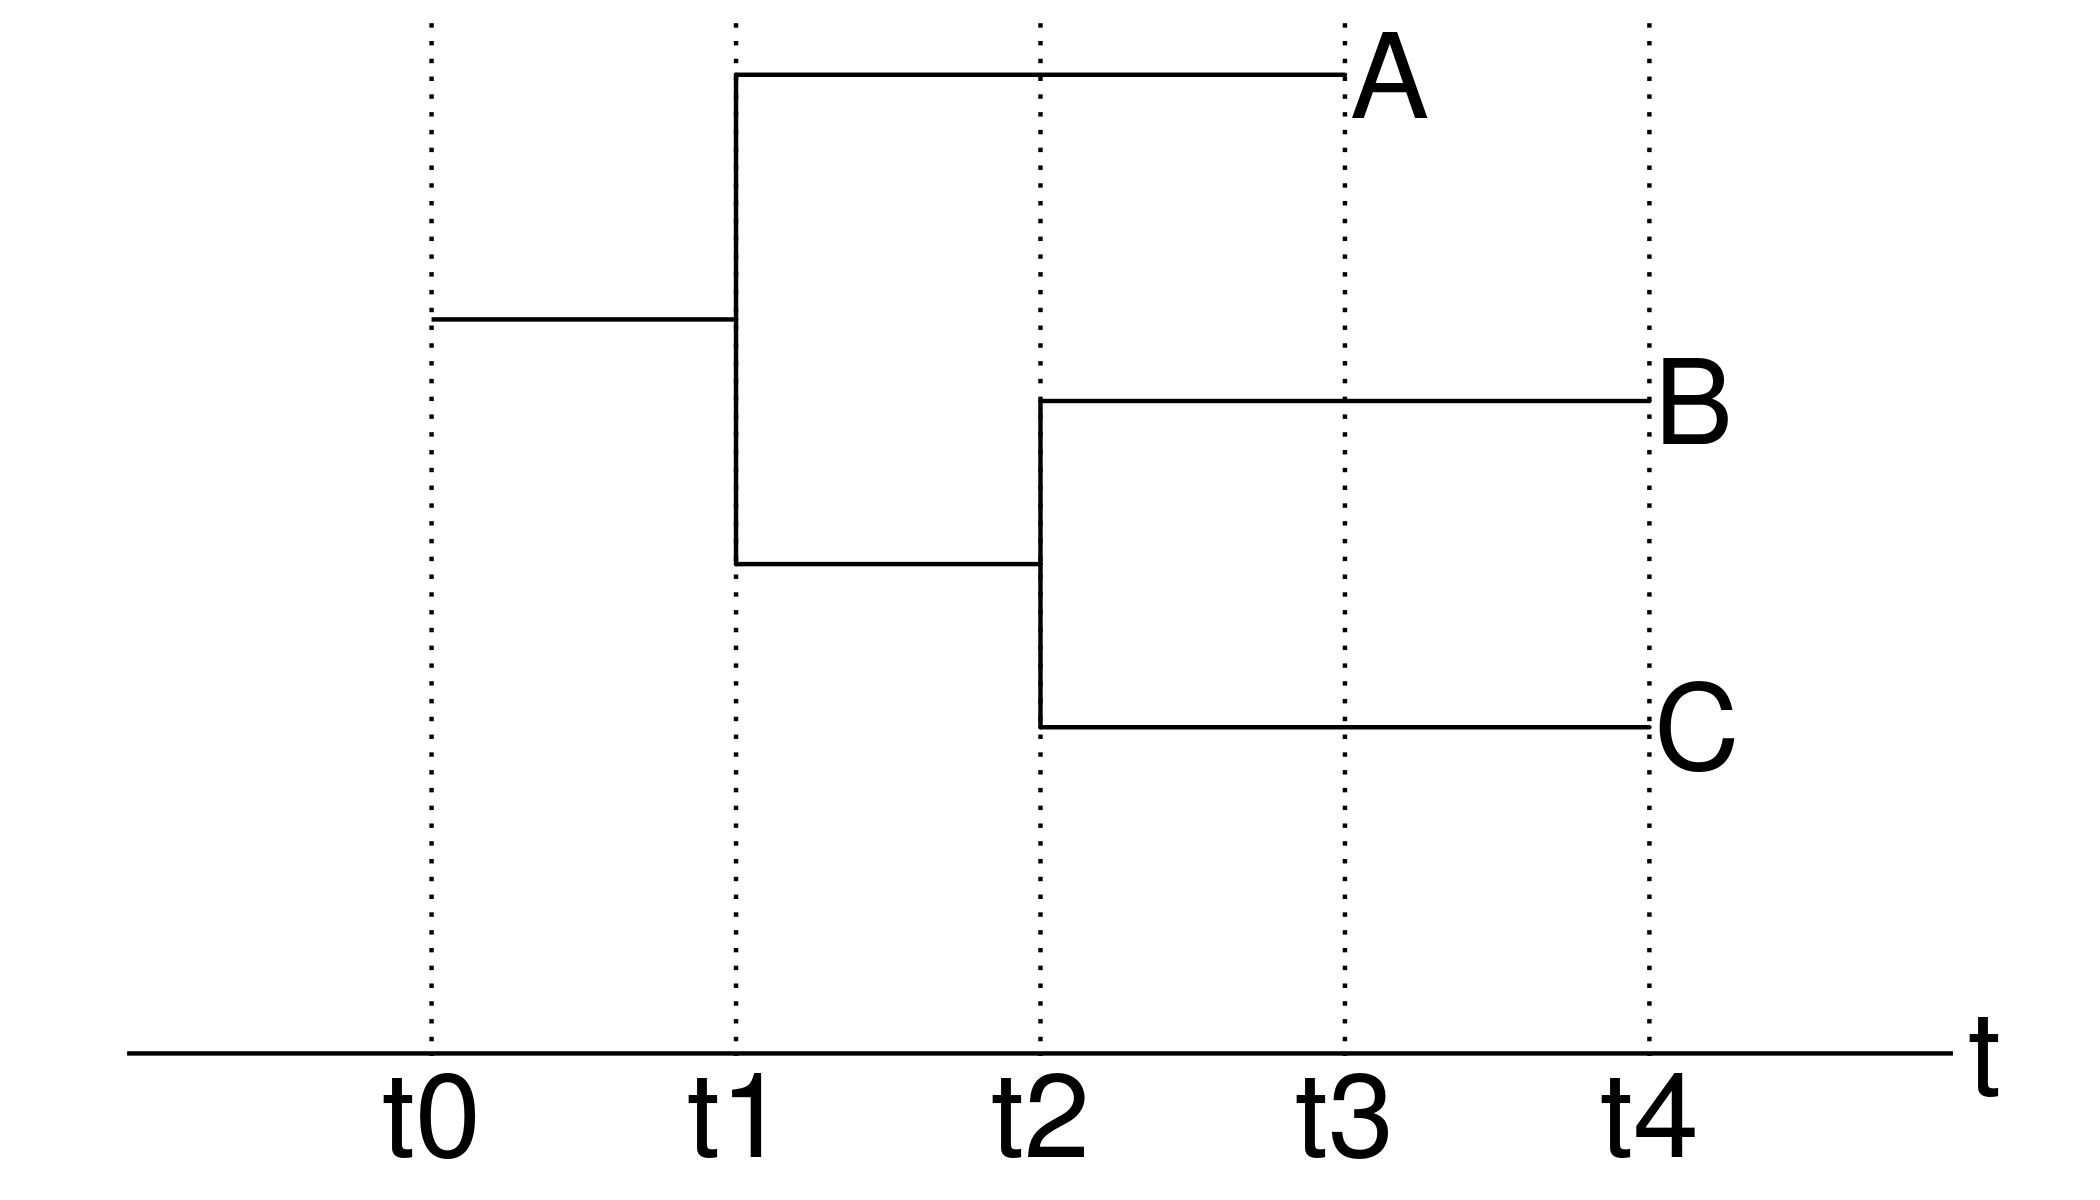
\includegraphics[width=0.3\textwidth]{t_3.png}
  %
  %     +--------x   A
  %  ---+     
  %     |     +------- B
  %     +-----+
  %           +------- C
  %
  % -+--+-----+--+---- (time)
  %  t0 t1    t2 t3
  %
  \caption{
    Evolutionary history of the three descendants of FUCA,
    of which one (A) went extinct.
    Assuming B and C gave rise to all contemporary biodiversity,
    the Last Universal Common Ancestor (LUCA) existed at timepoint t2. Time goes from past (left) towards the present (right).
  }
  \label{fig:t_3}
\end{figure}

The idea that all life on Earth is related was first posed by Charles Darwin in his book 'On the Origin of Species' 
in 1859 (\cite{darwin}).
His first sketch of an evolutionary tree is shown in figure 
\ref{fig:darwins_phylogeny}.

\begin{figure}[H]
  \includegraphics[width=0.3\textwidth]{Darwin_Tree_1837.png}
  \caption{
    Charles Darwin's first sketch of an evolutionary tree (1837).
  }
  \label{fig:darwins_phylogeny}
\end{figure}

The biodiversity derived from the first life on Earth 
is important to us humans (apart from that is has created us) for many reasons. One of these is that biodiversity usually improves ecosystem 
services (\cite{cardinale2012biodiversity}),
where ecosystem services are features of biological systems that are 
positive for human well-being, for example food,
carbon sequestration, waste decomposition and pest control. Therefore, biodiversity is linked to human well-being. Biodiversity is considered so important that the European Union has an explicit Biodiversity Strategy,
which aims to halt the loss of biodiversity (see 
  \url{https://ec.europa.eu/environment/nature/biodiversity/strategy/index_en.htm}
).

\begin{figure}[H]
  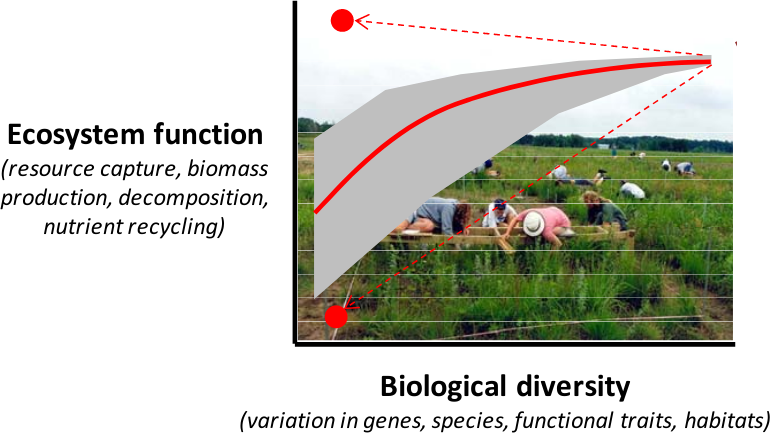
\includegraphics[width=0.5\textwidth]{cardinale_et_al_fig_1.png}
  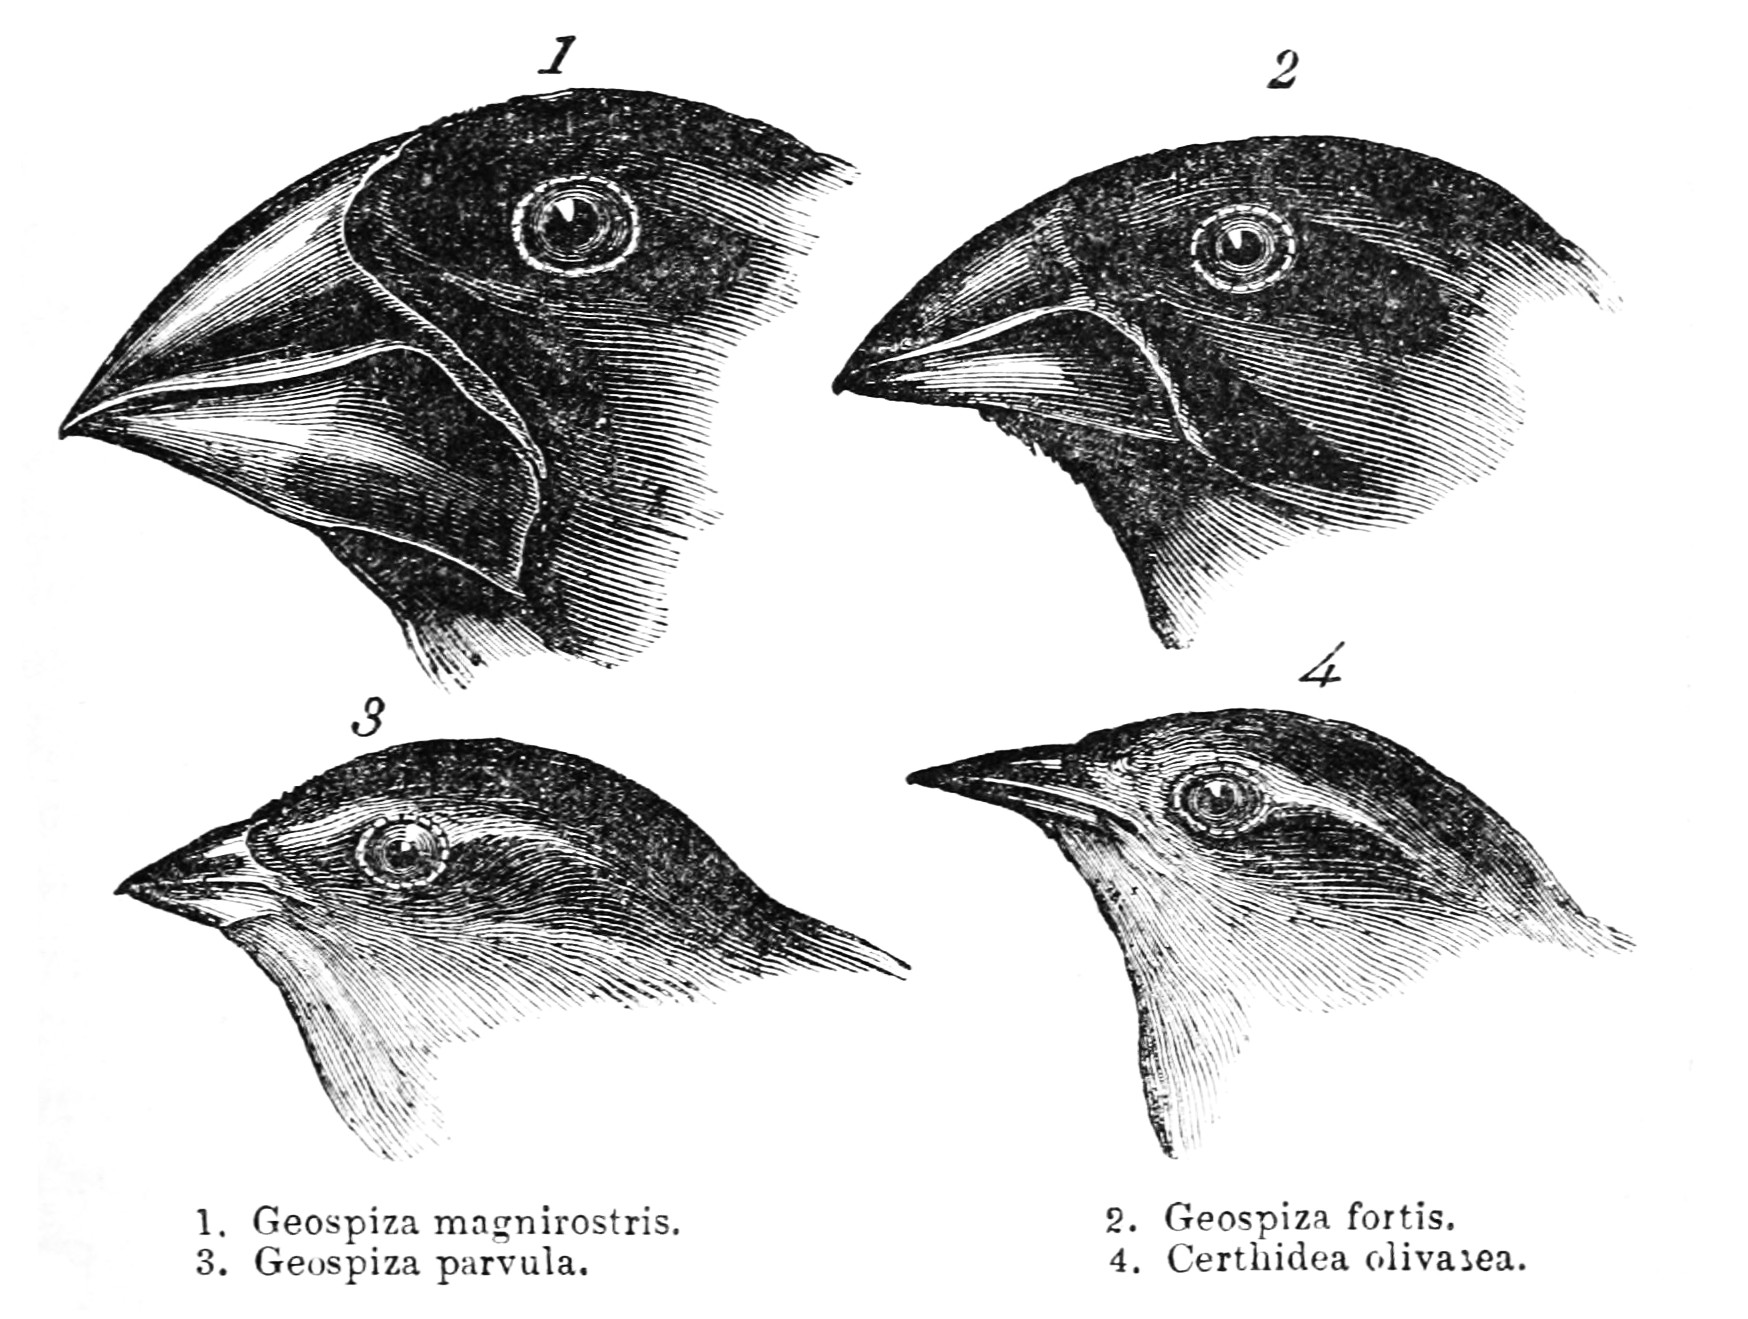
\includegraphics[width=0.5\textwidth]{Darwin's_finches_by_Gould.jpg}
  \caption{
    Left: a diversity-function relationship found to be typical from hundreds
    of studies. The red line represents an average, where the gray polygon
    represents a 95\% confidence interval. The red dots show the lower
    and upper limit for monocultures. From \cite{cardinale2012biodiversity}.
    Right: Darwin's finches, by John Gould.
  }
  \label{fig:cardinale_et_al_and_darwins_finches}
\end{figure}

Speciation is the process that increases biological diversity.
This process is studied from multiple angles; among others,
we can study the mechanism ('what
causes a speciation event?') or we can study the patterns of many
of such events ('is speciation rate constant through time?').
Darwin's finches (see figure \ref{fig:cardinale_et_al_and_darwins_finches}) 
represent an iconic example of speciation with 25,000 results on Google Scholar.
There are many suggested mechanisms underlying speciation events, such as reproductive incompatibilities arising in geographical isolation 
(e.g. \cite{mayr1942}), ecological factors (e.g. \cite{lack1947}) causing divergent selection, and sexual selection resulting in assortative mating. However, listing and explaining all mechanisms is beyond the scope of this thesis. In this thesis I assume speciation occurs and I focus on the questions what impact it has on evolutionary relationships between species and how we can infer speciation events from observed evolutionary relationships, as encoded in a phylogenetic tree. Getting such a phylogeny is not trivial, as I will discuss below. But once we have such a phylogeny, we can ask many question such 
as 'How often do speciation and extinction events take place?'
'Are speciation and extinctions rates constant, or do they change?',
'What causes a change in the speciation rate or the extinction rate?' or
'Is there an upper limit to the number of species?'. 

There are two methods to study speciation patterns in evolutionary time:
the use of fossils or the use of molecular phylogenies.

\begin{figure}[H]
  %
  % [picture of El Graeco fossil] | [](800px-Hominini_lineage.svg.png), from https://en.wikipedia.org/wiki/File:Hominini_lineage.svg
  %                               | 
  %  El Greaco                    | HS     Pan
  %                               |  \    /
  %                               |   \  /
  %                               |    \/
  %                               |     \
  %
  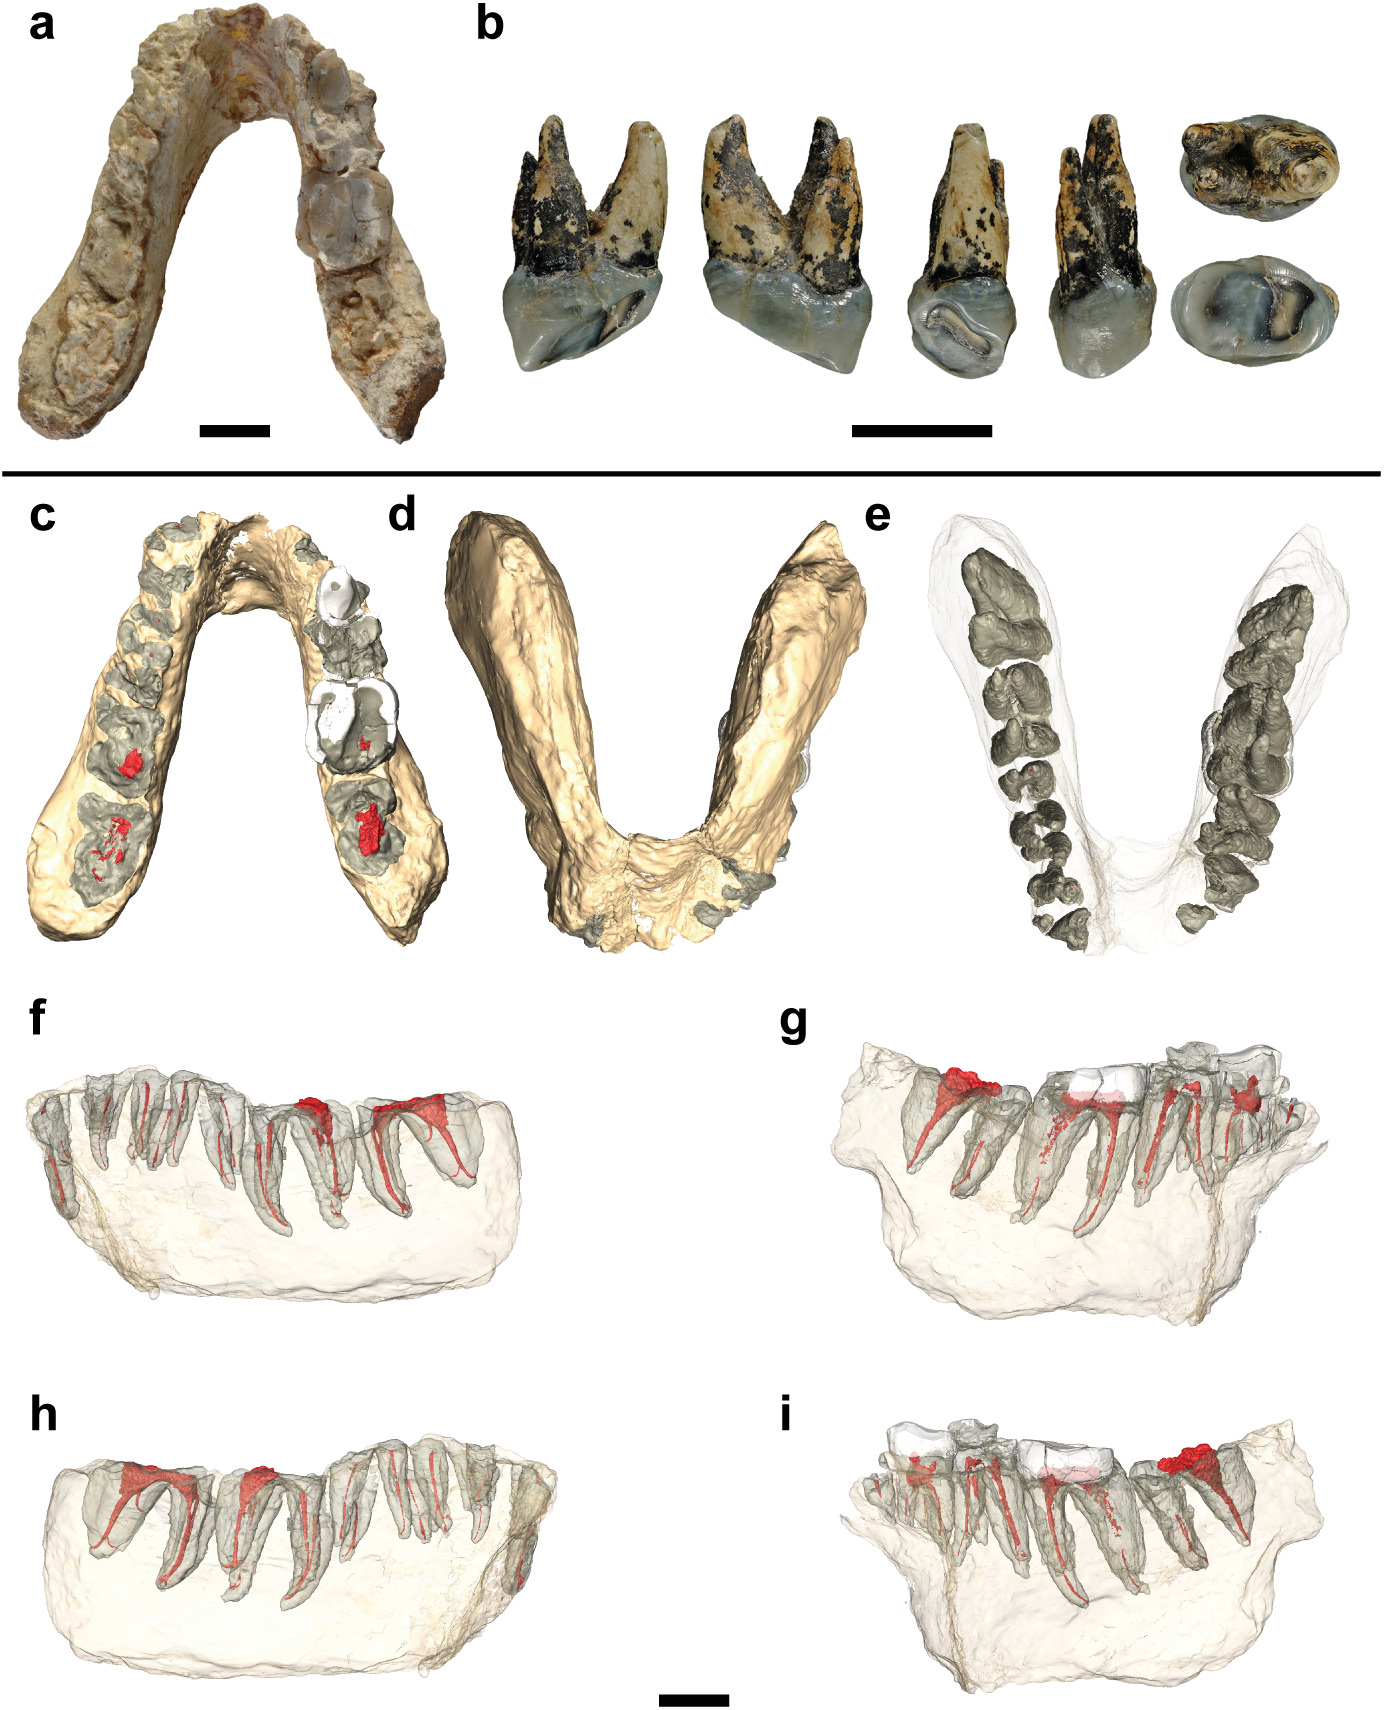
\includegraphics[width=0.3\textwidth]{Graecopithecus.jpg}
  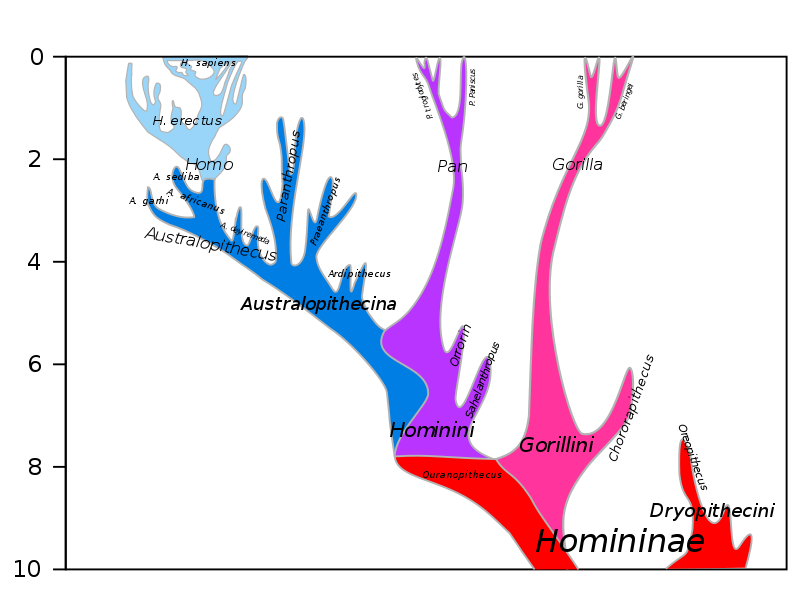
\includegraphics[width=0.5\textwidth]{Hominini_lineage.png}
  \caption{
    Left: El Graeco fossil, from \cite{fuss2017potential}.
    Right: Evolution of the Homininae, based on \cite{stringer2012makes}
 }
  \label{fig:human_evolution}
\end{figure}

Using fossils is a classic way to look back in evolutionary time.
Fossils show a glimpse of the biodiversity in the past.
We can deduce the age of fossils, by dating the rock layers they are found in.
Using fossils has its limitations. First, it is mostly species with hard body
parts that fossilize. Even in such species, organisms are 
only rarely preserved, and only a fraction of preserved fossils are preserved under ideal circumstances. Of 
these fossils, only a fraction is discovered.
One example of a famous fossil is 'El Graeco', 
which may be the oldest known hominin (\cite{fuss2017potential}), where
hominins are the tribe (taxonomic group) we Homo sapiens share with the Panini.

\begin{figure}[H]
  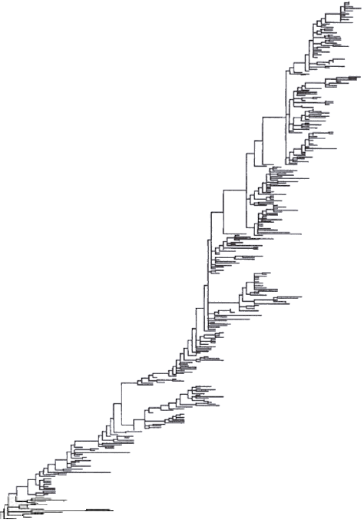
\includegraphics[width=0.3\textwidth]{bush_et_al_1999}
  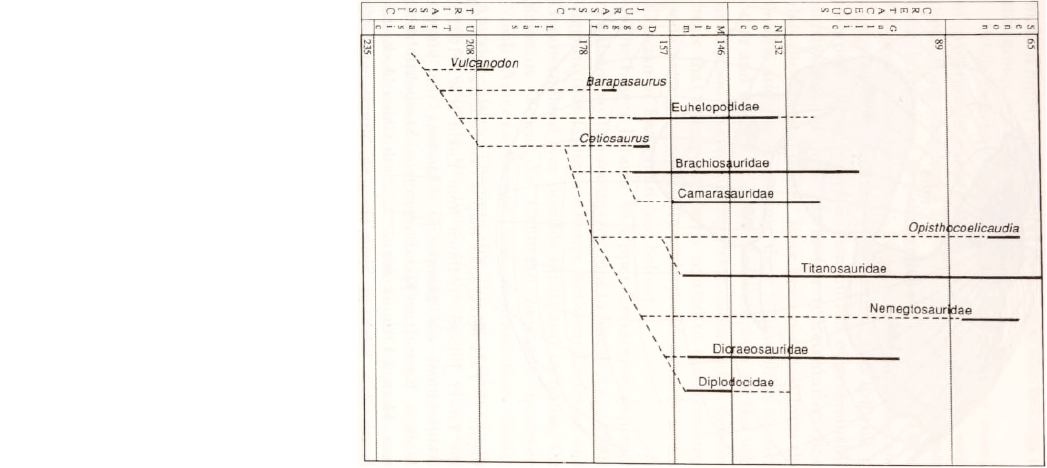
\includegraphics[width=0.7\textwidth]{dinosaur_phylogeny.png}
  \caption{
    Left: phylogeny of the human influenza virus type A subtype H3,
    from \cite{bush1999positive}.
    Right: the evolutionary history of sauropod dinosaurs,
    from \cite{upchurch1995evolutionary}
  }
  \label{fig:bush_et_al_1999}
\end{figure}

Using molecular phylogenies is the modern way to look back in evolutionary time.
It is the use of heritable molecules (for example DNA, RNA, or proteins)  
of contemporary species to infer phylogenies. 
The field of phylogenetics is the research discipline that
intends to infer the most accurate phylogenies possible, 
regarding topology, speciation and extinction times,
optionally adding morphological data and/or fossil data.
Phylogenetics is applied in many settings, among
others, species classification,
forensics, conservation ecology
and epidemiology (\cite{lam2010use}).

One example of the importance of an accurate phylogenetic tree 
is demonstrated in \cite{bush1999positive}. This study
investigated which loci of the H3 hemagglutinin surface protein
are under selection, by contrasting nonsynonymous and synonymous
mutation rates along the branches of a phylogeny. 
They noted that
most selection rates were either below or above the 
statistical threshold depending on the phylogeny.
This study contributed to recommendations on the 
composition of influenza virus vaccines.

\begin{figure}[H]
  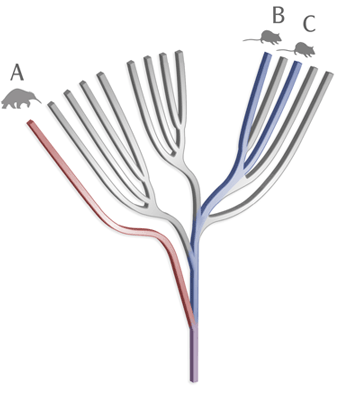
\includegraphics[width=0.3\textwidth]{edge_tree.png}
  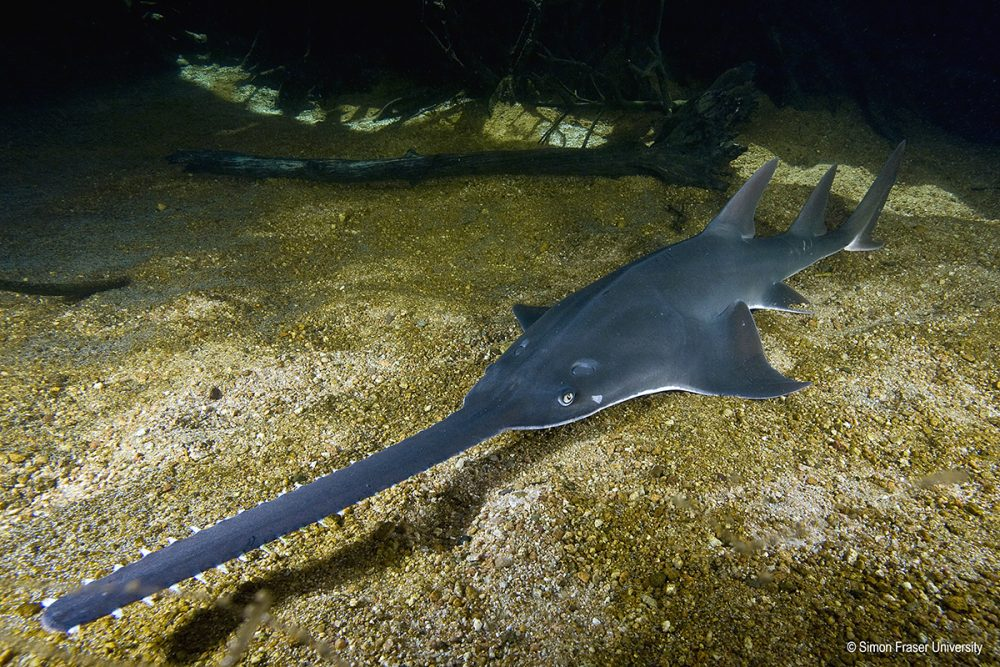
\includegraphics[width=0.5\textwidth]{Pristis-pristis_Simon-Fraser-University-1000x667.jpg}
  \caption{
    Left: The ED (evolutionary distinctiveness)       
    of species A is higher than that of species 
    B or C, as more                             
    evolutionary history will be lost when      
    that species goes extinct.
    Right: The Largetooth Sawfish (Pristis pristis) is at number 1 of the 
    EDGE (ED = 'Evolutionary Distinctiveness', GE = Globally Endangered status) 
    list, with an EDGE Score of 7.38 and an ED of 99.298.
 }
  \label{fig:edge_species}
\end{figure}

Another example of the importance of an accurate phylogenetic tree 
comes from conservation biology, in which phylogenies are used to
calculate an EDGE ('Evolutionarily Distinct and Globally Endangered') 
score. Species with a high EDGE score are prioritized in conservation.
To calculate an EDGE score, one needs a metric of evolutionary 
distinctiveness ('ED') and globally 'endangeredness' ('GE').
The GE score is a conservational status, ranging from zero ('Least Concern') 
to four ('Critically Endangered'). 
The ED embodies the amount of evolutionary history lost if the species 
went go extinct, which can be calculated from a (hopefully accurate) 
phylogeny.

Phylogenetics has taken a huge flight, due to the massively increased
computational power and techniques. A first milestone in this field is 
the work of Felsenstein in 1980, creating (and still maintaining!) 
PHYLIP (\cite{felsenstein1981evolutionary}), 
the first software package for classical phylogenetic analysis.
Another milestone is the Metropolis-Hasting algorithm, which 
allowed Bayesian phylogenetics to thrive, resulting in
contemporary tools such as BEAST (\cite{beast1}), BEAST2 (\cite{beast2}) (of which more below), 
MrBayes (\cite{mrbayes}) and RevBayes (\cite{revbayes}).

\begin{figure}[H]
  
\includegraphics[width=0.2\textwidth]{phylip.png}
  
\includegraphics[width=0.2\textwidth]{beast_logo.png}
  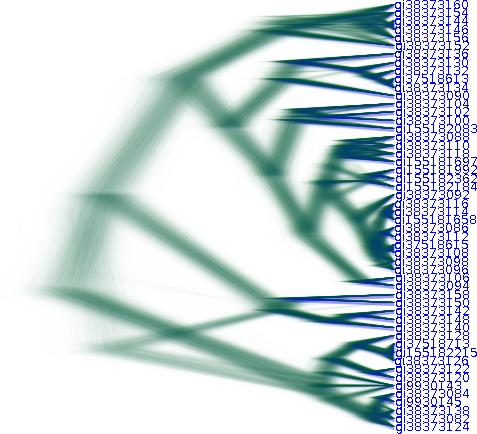
\includegraphics[width=0.2\textwidth]{DensiTreeExample2.jpg}
  \caption{
    Left: PHYLIP logo. 
    Center: BEAST2 logo.
    Right: BEAST2 example output
  }
  \label{fig:beast2}
\end{figure}

A clear example of the power of modern phylogenetics,
is the Tree Of Life.
The Tree Of Life is based on the proteome of 3,083 species.
A proteome of a species consists of all the proteins found within that species.
To be able to compare between different species, the researchers
used part of the proteome that is common in most of these species,
which consisted of 2,596 amino-acids.
To create the Tree of Life, it took 3,840 computational hours on a modern 
supercomputer (\cite{hug2016new}).

\begin{figure}[H]
  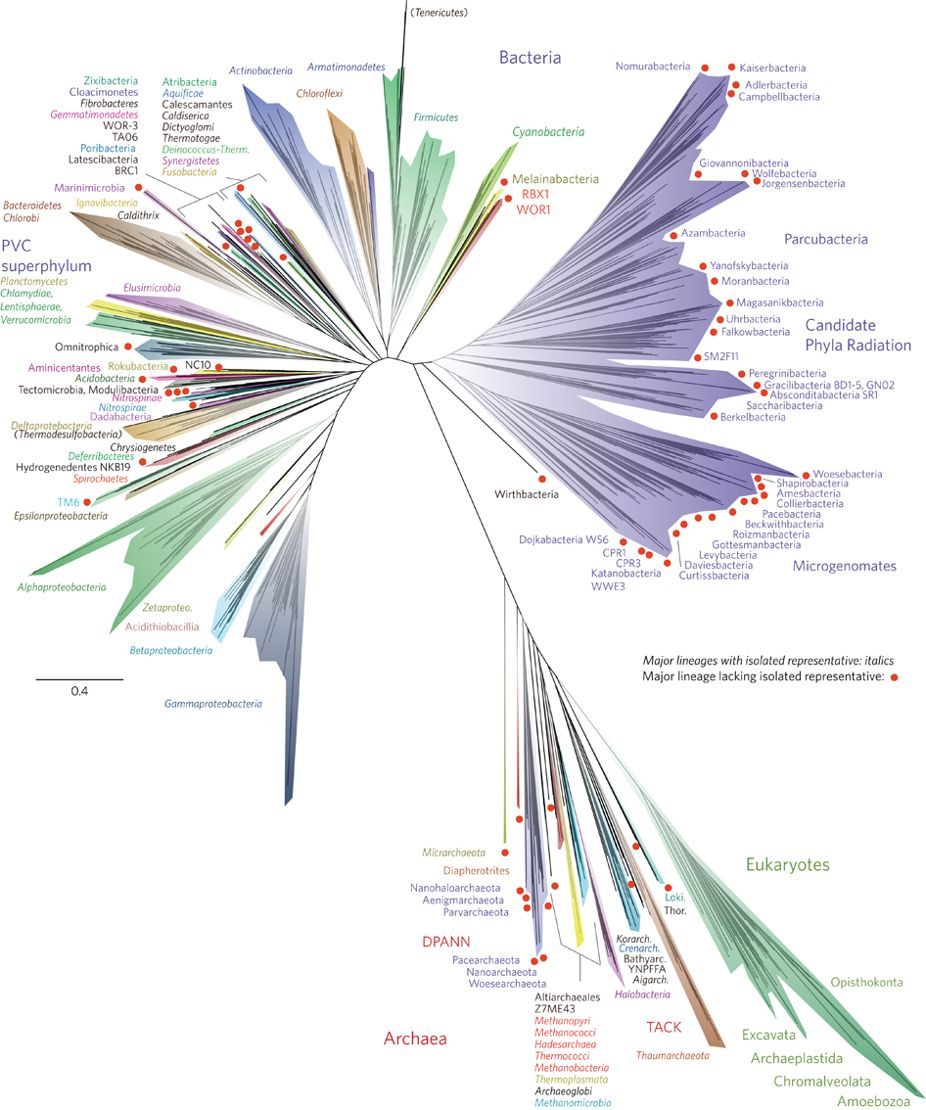
\includegraphics[width=0.4\textwidth]{tree_of_life_2016.jpg}
  \caption{
    Tree of Life, from \cite{hug2016new}
 }
  \label{fig:tree_of_life}
\end{figure}

To create such a tree from protein sequences, one has to specify
an evolutionary model. This evolutionary model embodies our set of
assumptions,
such as the way a protein sequence evolves (also called the site model), 
the rate(s) at which this happens (the clock model) 
and the way in which a branching/speciation event takes 
place (the tree model). 
For example, the amino acids of the Tree Of Life are assumed to change
over time according to the LG model (\cite{le2008improved}).
The speeds at which amino acids change to others are called the transition
rates. The LG model is a model for amino acid transitions, 
which uses the average rates found in nature.

There are many evolutionary models to choose from, 
and selecting which one to use is hard, due to the many sets of assumptions
to choose from. In general, modelers are looking for that set of assumptions
that is as simple as possible, but not simpler. And even then, sometimes
an overly simplistic model is still picked, due to computational 
constraints. 

Ideally, one would like to have a rational way to select 
an evolutionary model that is as simple as possible, but not simpler.
Model comparison algorithms have been developed that select the evolutionary model that is
most likely to have generated the data, without being overly complex.
The idea is that the best evolutionary model should result in the
most accurate phylogenetic trees.

Because model comparison is hard, there have been multiple
studies investigating the effect of picking the wrong
evolutionary models. 

\begin{figure}[H]
  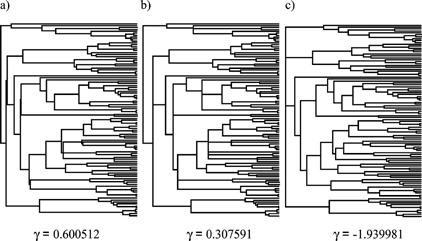
\includegraphics[width=0.7\textwidth]{revell2005under.png}
  \caption{
    Figure from \cite{revell2005under}. Left: true tree. Middle: inferred tree, inferred using the generative model (i.e. the model that generated the true tree)
    Right: inferred tree, inferred using an inference model that is simpler than the generative model
 }
  \label{fig:revell2005under}
\end{figure}

One example that demonstrates the effect of using a too simple inference model
is provided by Revell and colleagues (\cite{revell2005under}).
They first simulated many phylogenies.
From those phylogenies, they simulated DNA sequences for each of
the virtual species.
DNA is the heritable material all life on Earth possesses,
which consists of a sequence of the four DNA nucleotides.
In the simulation of the DNA sequences, the experimenters
used different DNA substitution models.
A DNA substitution model embodies the transition rates of these nucleotides (see
figure \ref{fig:dna_substitution} for an example).
From the simulated DNA sequences, the researchers inferred phylogenies again,
with either the correct or a simpler DNA substitution model.
Ideally, the inferred phylogenies match the phylogenies the alignments are based upon.
They found that when the DNA model is the correct one, inference of the
phylogenies is not flawless but satisfactory.
However, when using an overly simplistic DNA model, 
the inferred tree shows a slowdown in their speciation rates, 
even when the original tree was simulated with a constant speciation rate.
This study shows that a decreasing speciation rate may be attributed
to an overly simplistic DNA model, instead of an interesting biological process.

\begin{figure}[H]

  %
  % n_lineages
  %
  %   |      _______________
  %   |   __/
  %   | _/
  %   |/
  %   +---------------------
  %
  %       time
  %
  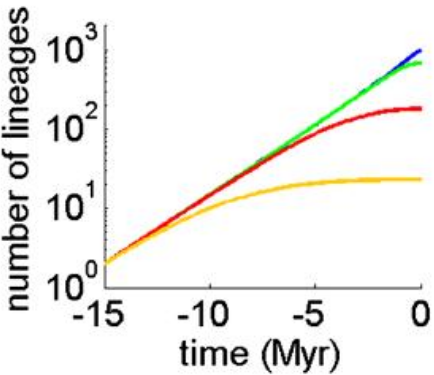
\includegraphics[width=0.3\textwidth]{etienne_rosindell_2011_ltt.png}
  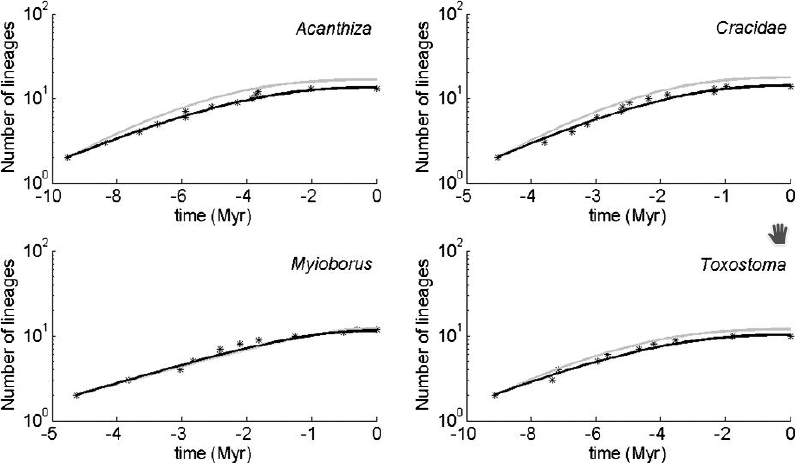
\includegraphics[width=0.5\textwidth]{etienne_rosindell_2011.png}
  \caption{
    Left: example lineage-through-time plots, for different 
    speciation completion rates: yellow = 0.01, red = 0.1, green = 1.0, blue = 10.
    Note the slowdown in the accumulation of new lineages when speciation completion
    rate is lowered.
    Right: number of species through time plots for four bird phylogenies, 
    (after \cite{phillimore2008density})
    Both figures are adapted from \cite{etienne2012prolonging}
 }
  \label{fig:etienne2012prolonging}
\end{figure}

A more recent example that demonstrates the effect of using an overly simple 
inference model is the study by Duchêne and co-workers (\cite{duchene2014impact}),
who looked into the consequences of assuming a wrong clock model. 
A clock model embodies our assumptions regarding the mutation rates in
the histories of different taxa. The simplest clock model, called the strict
clock model, assumes these mutation rates are equal across all taxa.
Using a wrong clock model has a profound impact 
on the inferred phylogenetic trees, unless we can
specify the timing of some early speciation 
events (\cite{duchene2014impact}).

\begin{figure}[H]
  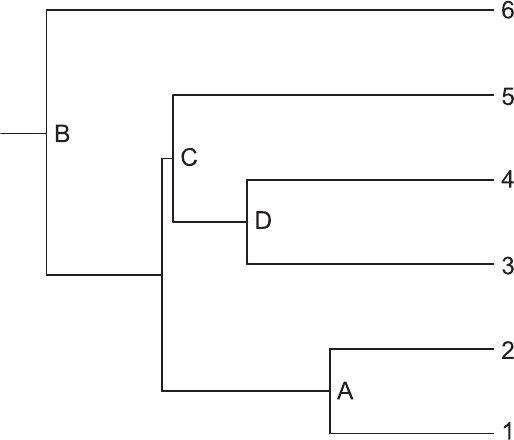
\includegraphics[width=0.3\textwidth]{duchene_et_al_2014_fig_1.png}
  \caption{
    Phylogeny with speciation events labelled A to D,
    where B is the earliest speciation event.
    Figure from \cite{duchene2014impact}.
 }
  \label{fig:duchene2014impact}
\end{figure}

The tree model is the most important part of the evolutionary model needed for phylogenetic inference,
with regard to speciation. The assumptions of a tree model are collectively 
called the tree prior, where 'prior' refers to the knowledge
known before creating a phylogeny. The tree prior specifies the probability of
processes that determine the shape of a tree. These
two processes are (1) the formation of a new branch, 
and (2) the termination of
an existing branch. In the context of speciation, we call these
two events a speciation and an extinction event respectively.

There are two standard tree models, called the Yule
and Birth-Death model. The most basic speciation model
is the Yule model (\cite{yule1925mathematical}), 
which assumes that speciation
is constant and there is no extinction.
Although extinction is a well-established phenomenon, 
the utility of the Yule model is its simplicity: it is the
simplest evolutionary model to work with, and the computation
of the probability of a tree under the Yule process is very fast,
making it a good first step in an evolutionary experiment.
Similar to the simplest models of bacterial growth,
the Yule model predicts that the expected number of species 
grows exponentially through time.
Because the Yule model 
was later classified as a Birth-Death model without extinction,
it is nowadays also called the Pure-Birth model.

\begin{figure}[H]
  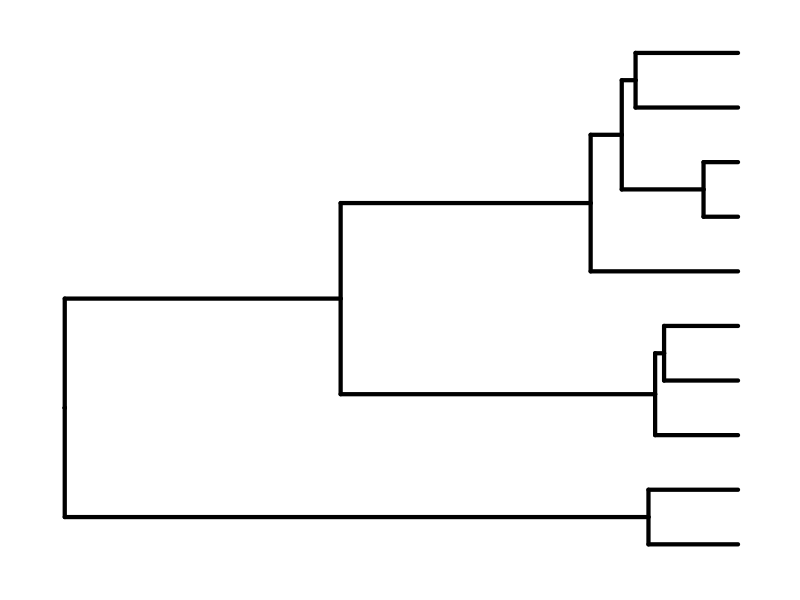
\includegraphics[width=0.4\textwidth]{yule_tree.png}
  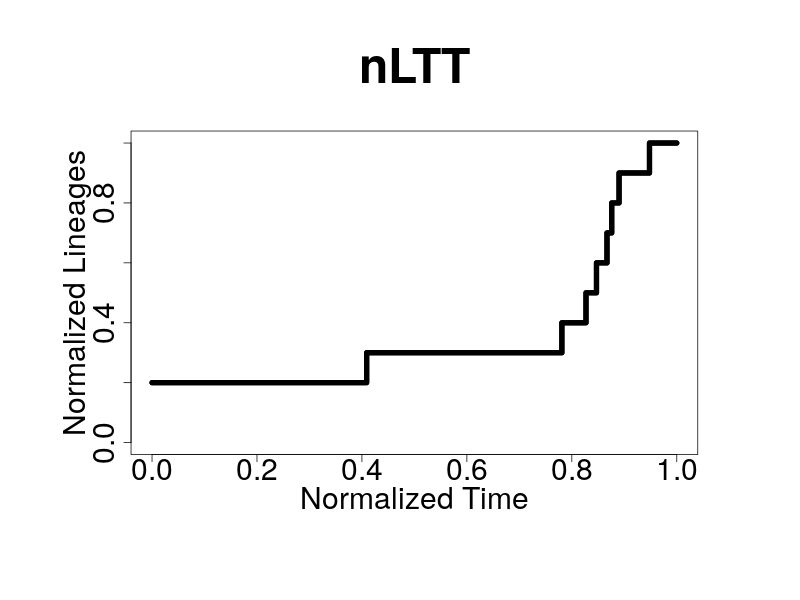
\includegraphics[width=0.4\textwidth]{yule_tree_nltt.png}
  \caption{
    Left: An example Yule tree
    Right: A lineages-through-time plot of the example Yule tree.
    In all cases, time goes from past (left) towards the present (right).
  }
  \label{fig:yule}
\end{figure}

The Birth-Death model (\cite{nee1994}) is an extension of the
Yule model, as it adds extinction.
Similar to the constant birth rate, the extinction rate is assumed
to be constant as well.
As a consequence, the BD model predicts two outcomes:
if the speciation rate exceeds the extinction rate,
the expected number of extant species grows exponentially through time. 
The other way around, however, when the extinction rate exceeds
the speciation rate, the expected number of lineages is expected to decline
exponentially.
It is clear that exponential growth in the expected number of lineages
is biologically nonsensical. 
To state the obvious: a finite area (Earth) results in a finite number of species. 
Applying the BD model to molecular data already shows that it does not
always hold, as shown by figure \ref{fig:bd}.

\begin{figure}[H]
  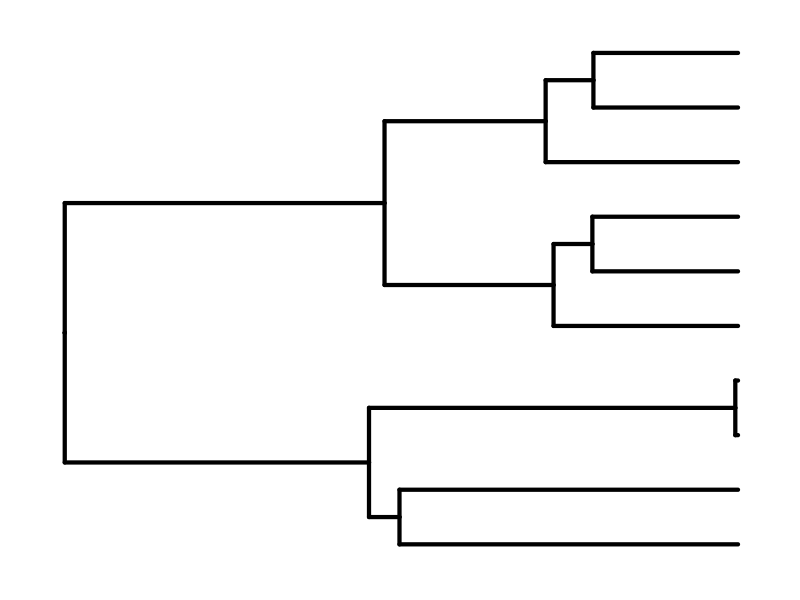
\includegraphics[width=0.4\textwidth]{bd_tree.png}
  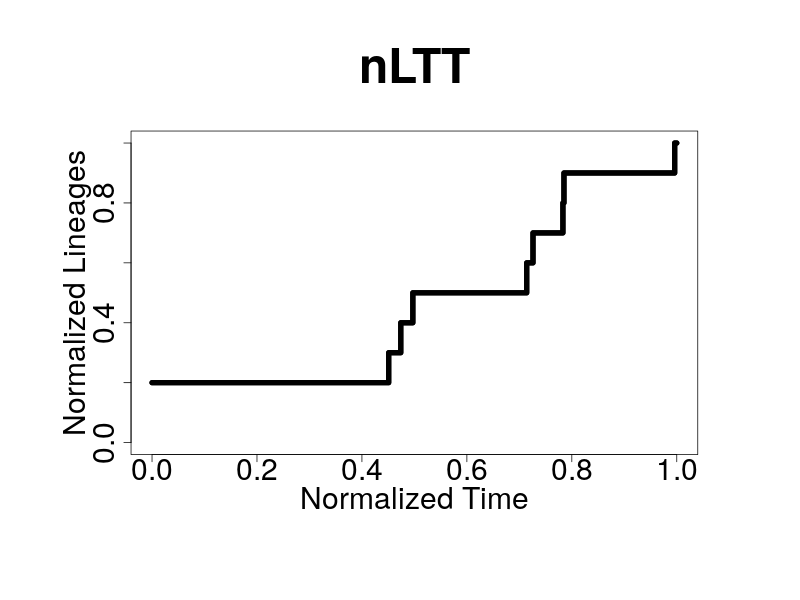
\includegraphics[width=0.4\textwidth]{bd_tree_nltt.png}
  \caption{
    Left: An example Birth-Death tree
    Right: A lineages-through-time plot of the example Birth-Death tree.
    In all cases, time goes from past (left) towards the present (right).
  }
  \label{fig:bd}
\end{figure}

\begin{figure}[H]
  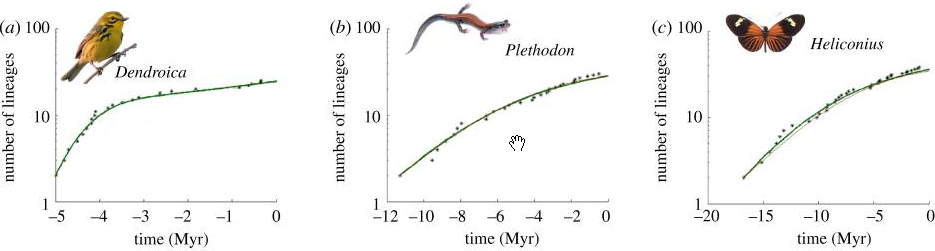
\includegraphics[width=0.8\textwidth]{etienne_et_al_2012_dd_1.png}
  %
  % n_lineages
  %
  %   |      _______________
  %   |   __/
  %   | _/
  %   |/
  %   +---------------------
  %
  %       time
  %
  \caption{
    An LTT plot for bird/lizards showing a slowdown in speciation
    rate, adapted from \cite{etienne2012diversity}. Because the number
    of lineages on the y-axis are plotted on a logarithmic scale,
    exponential growth would show as a straight line. 
  }
  \label{fig:bd}
\end{figure}

A recent study investigating the effect of picking
a wrong standard tree prior was provided by Sarver and 
colleagues (\cite{sarver2019choice}).
In this study, they first simulated trees using either a Yule or a birth-death
tree model, after which they simulated an alignment from that phylogeny
using two different standard clock models. From these alignments, 
they inferred the original trees using all of the four 
different clock and tree prior combinations. 
They showed that, regardless of which priors are used,
the estimated speciation and diversification rates 
from the inferred trees are similar to those of the original tree.

\begin{figure}[H]
  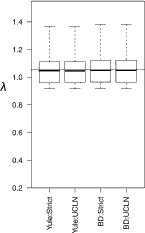
\includegraphics[width=0.2\textwidth]{sarver2019choice_top_4_bars.png}
  \caption{
    Estimation of the speciation rate ($\lambda$)
    on inferred trees using 4 evolutionary models.
    The original trees had 100 taxa and were simulated with a strict clock model 
    and BD tree model, with a speciation rate of 1.104.
    Adapted from \cite{sarver2019choice}.
 }
  \label{fig:sarver2019choice}
\end{figure}

This thesis investigates the effect of picking a wrong standard
tree prior, when the tree is generated by a non-standard, novel tree model.
I will describe one new biologically relevant tree model, as well as the re-usable framework to determine the effect of using a standard tree prior. 

This novel and non-standard tree model is the multiple-birth 
death (MBD) model by Laudanno and colleagues (unpublished).
While the standard BD models assume that a speciation event occurs in one
species only at a time, the MBD models allows for speciation events
to occur in multiple species at the same time.
The biological idea behind this model, is that when a 
habitat (lake or mountain range) gets split into two, 
this may trigger speciation events in both communities at the same time. 
This mechanism is posed as an
explanation for high biodiversity in the African rift lake Tanganyika,
where the water level rises and falls with ice ages,
splitting up and merging the lake again and again, 
triggering co-occurring speciation events at each change. 

%
% [phylogeny from Lake Tanganyika, use reference from Giovanni's MBD article]
%
% Phylogeny from Lake Tanganyika
%

This thesis investigates the effect of picking a wrong standard
tree prior, when the tree is generated 
by a non-standard tree model, using the phylogenetic software 
called BEAST2 (\cite{beast2}),
an abbreviation of 'Bayesian Evolutionary Analysis by Sampling Trees'.

\begin{figure}[H]
  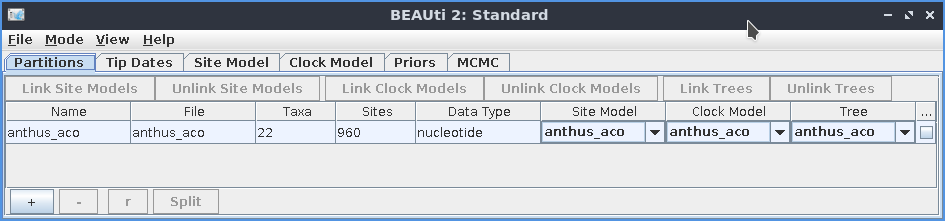
\includegraphics[width=0.5\textwidth]{beauti_alignment.png}
  \caption{
    BEAUti, after having picked a DNA alignment
  }
  \label{fig:beauti_alignment}
\end{figure}

We chose to use BEAST2 (\cite{beast2}) over other phylogenetic software,
because BEAST2 is popular, beginner-friendly, flexible, has a package manager
and a modular well-designed software architecture. The beginner-friendliness
comes from the BEAST2 program called BEAUti, in which the user can set up
his/her evolutionary model from a graphical user interface. There are many (in
the order of dozens to hundreds) options to set up an evolutionary inference model. 
These choices are categorized in a site model, clock model and a tree prior. 

\begin{figure}[H]
  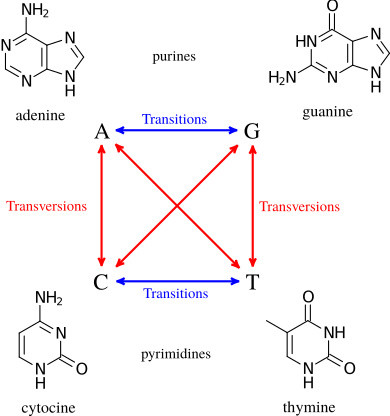
\includegraphics[width=0.5\textwidth]{transitions_and_transversions.png}
  \caption{
    Classification of nucleotide substitutions. The simplest nucleotide
    substitution model (JC69) assumes all 6 rates are equal, whereas
    the most complex one (GTR) allows all of these to differ.
 }
  \label{fig:dna_substitution}
\end{figure}

A site model embodies the way the characters - nucleotides in our case of DNA sequences -
change over time. One can specify the proportion of nucleotides
that changes, or let it be estimated. Furthermore, one can specify how dissimilar different transition
rates may be between different nucleotides. Most essential is the nucleotide
substitution model, which entails the relation between the twelve transition 
rates from any of the four nucleotides to any of the other three nucleotides. 
The simplest model (called
JC69) assumes all are equal, whereas the most complex model (called GTR) assumes
that all may differ. The standard BEAST2 software has four site models, but there is a BEAST2 
package that contains 18 additional nucleotide substitution models.

\begin{figure}[H]
  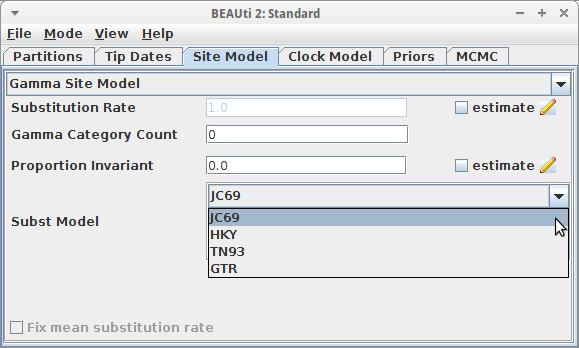
\includegraphics[width=0.5\textwidth]{beauti_site_model.png}
  \caption{
    Specifying a site model in BEAUti
 }
  \label{fig:beauti_site_model}
\end{figure}

To give an idea of the flexibility of BEAST2, I will zoom in on specifying
one simple aspect of the inference model: the proportion invariants.
The proportion invariants is the proportion, ranging from a value of zero (for 'none') 
to one (for 'all'), of nucleotides that remains unchanged throughout
the evolutionary history. This proportion can either be set to a certain 
value, or be estimated. If the value is set to a certain value, BEAST2 assumes
this as the truth. If the value is to be estimated by BEAST2, then
one must additionally specify an initial value and 
a distribution how probable the different values are. 
By default, BEAST2 assumes a uniform distribution,
that assigns an equal probability to all values between (and including)
zero and one. Instead of using a uniform distribution, 
there are ten other distributions that can be picked as well, allowing, for
example, to assign higher probabilities to certain proportions. 
So, for one simple value, there is already
a plethora of options, and there are even more that I will not discuss. 
Within BEAST2, this liberty is the rule, instead of the
exception, rendering it very flexible.

The clock model embodies how the mutation rates vary between
different species. The simplest clock model, called the strict clock,
assumes that mutation rates are identical in all species at all times. 
Two models (called relaxed-clock models) assume that mutation rates
between species are independent (yet all rates are from one probability 
distribution), but stay constant after each species' inception.
The last standard clock model (called a random local clock) assumes 
that all species have the same mutation
rate at any time, yet the mutation rates varies through time.

\begin{figure}[H]
  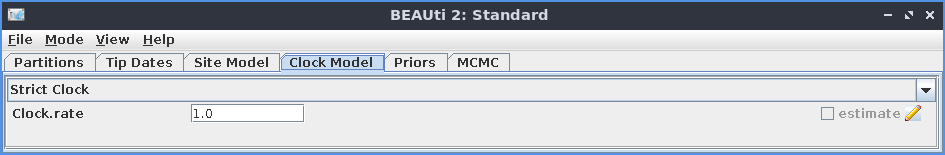
\includegraphics[width=0.8\textwidth]{beauti_clock_model.png}
  \caption{
    Specifying a clock model in BEAUti
 }
  \label{fig:beauti_clock_model}
\end{figure}

The tree prior specifies how a tree is built up, or, in our context,
how speciation takes place in time, at the macro-evolutionary level.
In our context, these are the Yule and Birth-Death model, which I already
described earlier.

\begin{figure}[H]
  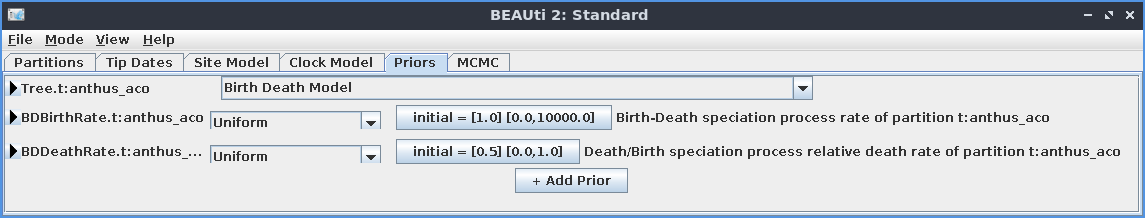
\includegraphics[width=0.8\textwidth]{beauti_tree_prior.png}
  \caption{
    Specifying a tree prior in BEAUti
 }
  \label{fig:beauti_tree_prior}
\end{figure}

This thesis investigates the effect of picking a wrong standard
tree prior, when the tree is generated 
by a non-standard tree model. 
It does so, by using the same experimental setup, called 'pirouette',
which is described in chapter 3. This framework is built up a foundation
of R packages called 'babette', which is described in chapter 2.

\begin{figure}[H]
  \includegraphics[width=0.3\textwidth]{The_Earth_seen_from_Apollo_17.jpg}
  \caption{
    Environment that follows an unknown speciation model.
 }
  \label{fig:unknown_speciation_model}
\end{figure}

In the end, we want to know how well we can infer a phylogeny from
molecular data found in the field. That field, outside, 
follows an unknown speciation model. Rather than just hope that our inference
is robust to whatever novel model we throw at it, with this thesis I have aimed at providing methodology that can assess that robustness.
